% This voodoo is needed for arXiv scripts and must appear within the first 4 lines
\pdfoutput=1
\documentclass[aps,prd,amsmath,floats,floatfix, twocolumn,
superscriptaddress,nofootinbib,showpacs]{revtex4-2}

% UTF8 always
\usepackage[T1]{fontenc}
\usepackage[utf8]{inputenc}
\usepackage{lmodern}
\usepackage{verbatim}
\usepackage[dvipsnames, usenames]{xcolor}
\definecolor{linkcolor}{rgb}{0.0,0.3,0.5}
\usepackage[hypertexnames=false, unicode, colorlinks=true, linkcolor=linkcolor,
citecolor=linkcolor, filecolor=linkcolor,urlcolor=linkcolor, pdfusetitle]{hyperref}

%\usepackage[colorlinks, pdfborder={0 0 0}, plainpages=false]{hyperref}
\usepackage[all]{hypcap}
\usepackage{graphicx}
\usepackage{xspace}
%\usepackage[usenames,dvipsnames]{color}
\usepackage{amssymb}
\usepackage[normalem]{ulem} %for \sout
\usepackage{bm} % boldmath
\usepackage{enumitem,amssymb}
\usepackage{orcidlink}
\usepackage{caption}
\usepackage{multirow}

% Better spacing
\usepackage{microtype}
\usepackage[english]{babel}
\usepackage{blindtext}

%
\graphicspath{%
  {figs/}%
  % More directories are added in braces, without commas between
}


\DeclareMathAlphabet{\mathpzc}{OT1}{pzc}{m}{it}

\newcommand{\roughly}{\mathchar"5218\relax\,} % Different from \sim in spacing
\newcommand{\into}{\!\times\!\relax} % Different from \times in spacing

% Macros for text changes
\newcommand{\red}{\textcolor{red}}
\newcommand{\blue}{\textcolor{blue}}
\newcommand{\green}{\textcolor{PineGreen}}
\newcommand{\nl}[1]{\textcolor{blue}{NL: #1}}
\newcommand{\ls}[1]{\textcolor{red}{[LS: #1]}}
\newcommand{\crp}[1]{\textcolor{magenta}[CP: #1]}
\newcommand{\ojp}[1]{\textcolor{orange}{OJP: #1}}
\newcommand{\Note}[1]{\textcolor{blue}{\textbf{[#1]}}}
\newcommand{\bfemph}[1]{\emph{\textbf{#1}}}
\newcommand{\TODO}[1]{\red{TODO: #1}}
\newcommand{\AddCite}{\red{[Needs citation]}}
\newlist{todolist}{itemize}{2}
\setlist[todolist]{label=$\square$}
\newcommand{\txt}[1]{{\textrm{\tiny{#1}}}}


% macros
\def\gw{gravitational wave\xspace}
\def\gwh{gravitational wave\xspace}
\def\gws{gravitational waves\xspace}
\def\GW{Gravitational Wave\xspace}
\def\GWs{Gravitational Waves\xspace}
\def\cw{continuous wave\xspace}
\def\cws{continuous waves\xspace}
\def\cwh{continuous-wave\xspace}


\newcommand{\TFFT}{T_\text{FFT}}
\newcommand{\tfftmax}{T_\text{FFT,max}}
\newcommand{\Tobs}{T_\text{obs}}
\newcommand{\thetathr}{\theta_\text{thr}}
\newcommand{\bea}{\begin{eqnarray}}
\newcommand{\eea}{\end{eqnarray}}
\newcommand{\be}{\begin{equation}}
\newcommand{\ee}{\end{equation}}

\newcommand{\ogw}{\tilde{\omega}}
\newcommand{\lgw}{\tilde{l}}
\newcommand{\mgw}{\tilde{m}}
\newcommand{\fgw}{f_{\rm gw}}
\newcommand{\mbh}{M_{\rm BH}}
\newcommand{\mb}{M_{b}}
\newcommand{\dotf}{\dot{f}_{\rm gw}}
\newcommand{\CR}{\text{CR}}
\newcommand{\opt}{\text{opt}}
\newcommand{\crossover}{\text{crossover}}

\definecolor{dkgreen}{rgb}{0,0.6,0}
\definecolor{gray}{rgb}{0.5,0.5,0.5}
\definecolor{mauve}{rgb}{0.58,0,0.82}

\newcommand{\bet}{\ensuremath{\frac{96}{5}\pi^{8/3}\left(\frac{G}{c^3}\right)^{5/3}M^{5/3}_cf^{8/3}_0}}
\newcommand{\befact}{\ensuremath{\left(1-\frac{8}{3}\beta t}\right)}
\newcommand{\befactD}{\ensuremath{\left(1-\frac{8}{3}(\beta+\Delta\beta) t\right)}}
\newcommand{\mcsun}{\ensuremath{\frac{M_c}{10^{-2}M_{\odot}}}}
\newcommand{\ftwo}{\ensuremath{\frac{f_0}{200~Hz}}}
\newcommand\anu{\affiliation{OzGrav-ANU, Centre for Gravitational Astrophysics, Research School of Physics and Research School of Astronomy \& Astrophysics, The Australian National University, ACT 2601, Australia}}
\newcommand\INFNRoma{\affiliation{INFN, Sezione di Roma, I-00185 Roma, Italy}}
\newcommand\uib{\affiliation{IAC3–IEEC, Universitat de les Illes Balears, E-07122 Palma de Mallorca, Spain}}
%\usepackage[dvipsnames, usenames]{xcolor}


%%%%%%%%%%%%%%%%%%%%%%%%%%%%%%%%%%%%%%%%%%%%%%%%%%%%%%
\begin{document}

\title{A semicoherent resampling method for long-transient gravitational wave searches with applications to subsolar mass primordial black holes binaries}

\author{Neil Lu}
\email{neil.lu@anu.edu.au }
\anu

\author{Cristiano Palomba}
\INFNRoma

\author{Ornella J. Piccinni}
\uib

\author{Ling Sun}
\anu


\date{\today}

%==========================================================================
\begin{abstract}
Resampling is a method for removing a modeled phase evolution
from gravitational wave data, transforming a frequency-evolving
signal into a monochromatic one. We introduce a novel
implementation that evaluates the Fourier spectrum of the resampled data
directly with a type-I non-uniform fast Fourier transform (NUFFT). This implementation
can achieve speedups up to two orders of magnitude faster than some previous
implementations. Demonstrating the applicability of this technique, we
construct a semicoherent search for long-duration inspiral signals from subsolar mass
primodial black hole binaries. For a search over $40$--$60\,\mathrm{Hz}$ and chirp
masses $5\times10^{-4}$-$10^{-1}\,M_\odot$, a coherent duration of
$30\,\mathrm{s}$ the estimated horizon distance
exceeds the Galactic Centre and Andromeda for parts of the target chirp-mass range.
We discuss the computational costs of such a search and find they are realistic, 
in part due to the improved resampling algorithm. 
These results establish NUFFT-based resampling as a computationally efficient
and broadly applicable basis for searches for modeled, frequency-evolving
gravitational wave signals.
\end{abstract}

\maketitle

%==========================================================================
% \tableofcontents

\section{Introduction}
\label{sec:introduction}

A decade after the first direct detection of gravitational waves (GWs) \cite{LIGOScientific:2016aoc}, GW astronomy has become an established observational probe of compact-object astrophysics and strong-field gravity. The LIGO \cite{LIGOScientific:2014pky}, Virgo \cite{VIRGO:2014yos}, and KAGRA \cite{KAGRA:2020tym} detectors have detected hundreds of compact-binary coalescence signals, transforming the original discovery into a growing population of astrophysical sources \cite{LIGOScientific:2026wfs}. The currently observed catalog consists of compact binary mergers whose signal durations in the sensitivity band of ground-based interferometers are typically short, ranging from fractions to tens of seconds.

There is growing interest in transient GW signals that remain detectable for much longer times. These could be produced by novel sources; post-merger remnants of neutron-star mergers \cite{LIGOScientific:2017fdd, Grace:2023kqq}, during or in the aftermath of pulsar glitches \cite{Keitel:2019zhb, Haskell:2023exob}, low mass primordial black hole (PBH) binaries \cite{Miller:2024rca, Andres-Carcasona:2024jvz, Rodriguez:2026oyia}, or ultralight vector boson clouds around black holes \cite{Siemonsen:2019ebd, Jones:2023fzz, LIGOScientific:2025csr}. These signals offer substantial scientific opportunities, but their long duration also creates difficulties in the analysis of such signals. The computational cost of matched filtering, the conventionally used technique for detecting signals, and template-bank size can increase rapidly with the signal duration \cite{Owen:1998dk}.

A natural way to reduce this cost is to use semicoherent methods. Such methods are standard in searches for continuous gravitational waves (also referred to as continuous waves), where fully coherent integration over months or years is often computationally prohibitive. In a semicoherent search, the data are divided into shorter segments, a detection statistic is coherently computed in each segment, and the information from different segments is then combined incoherently, for reviews on these methods see \cite{Wette:2023dom, Tenorio:2021wmz}. This sacrifices phase coherence and reduces sensitivity, but can dramatically reduce computational cost and enable broader searches over otherwise inaccessible parameter spaces. Semicoherent methods have been used to search for both modelled \cite{Piccinni:2018akm, Prix:2011qv} and unmodelled \cite{Suvorova:2016rdc, Sun:2017zge, Macquet:2021ttqa} signals. 

Semicoherent methods require the data to remain confined within a single Fourier bin in each segment. For slowly evolving continuous-wave signals, such as from rotating neutron stars, this condition can be satisfied even for long coherence times as the frequency evolution is often small. For more rapidly evolving signals, however, the frequency evolution would demand short coherence lengths to ensure the signal remains confined to a single Fourier bin (whose width is the inverse of the coherence time), causing loss of sensitivity. This motivates a preprocessing step known as resampling that removes the expected frequency evolution before constructing the spectra for each segment. Given a known signal model, the time series can be resampled to remove the modeled frequency evolution, after which it will be monochromatic and remain confined within a Fourier bin. This enables semicoherent analysis with longer coherence duration and greater sensitivities. 

When searching over signal durations from $\mathcal{O}(10^2\,\mathrm{s})$ to $\mathcal{O}(10\,\mathrm{months})$ the computational cost is, as with continuous wave analysis, dominated by the generation of the resampled time series and the subsequent Fourier transforms. In this work, we present a resampling implementation which accelerates both the frequency correction step and the subsequent production of Fourier spectra. We demonstrate the applicability of this technique in searches for binary sub-solar mass black holes (BHs), potentially of primordial origin, which may have formed in the early Universe \cite{Carr:2023tpt}. Unlike astrophysical black holes formed through stellar collapse, binary primordial black holes could exist with sub-solar masses \cite{Carr:1975qj} and therefore emit signals with durations lasting from tens of seconds to years. Within audio-band gravitational wave detectors these systems would remain in their inspiral phase before merging at higher frequencies. 

The structure of the paper is as follows. In Sec.~\ref{sec:signal_model} we describe the signal model we use for subsolar mass black hole inspirals and review some of their basic properties. In Sec.~\ref{sec:methods} we detail a semicoherent search which can be used to search for the subsolar mass black hole inspirals and provide details on the use of NUFFTs in the search. In Sec.~\ref{sec:distance_sens} we analytically derive the horizon distance this semicoherent method could reach. In Sec.~\ref{sec:injection} we verify this horizon distance with a signal injections into detector noise. In Sec.~\ref{sec:cost} we discuss the computational cost of the semicoherent search. Finally we conclude and discuss future work in Sec.~\ref{sec:conclusion}. 

%==========================================================================
\section{Signal model}
\label{sec:signal_model}
We consider the inspiral of two sub-solar mass PBHs. Binaries with total masses less than $0.1 M_\odot$ remain in the inspiral regime within the sensitivity band of ground-based detectors and coalesce at higher frequencies. This can be seen by considering the gravitational wave frequency of the inner-most stable circular orbit (ISCO), defined to be the minimal radial distance beyond which no stable circular orbits are possible, after which the signal has definitively exited the inspiral regime:
\begin{gather}
    f_{\rm ISCO} \simeq 4400 \frac{M_\odot}{M_{\rm tot}} \, \mathrm{Hz} \, .
\end{gather}
Systems with chirp masses less than $0.1 M_\odot$ coalesce at frequencies much higher than those detectable in ground-based detectors. 

It is also useful to consider the signal durations of sub-solar mass PBHs. The inspiral evolution of binary black holes is described by Post-Newtonian (PN) theory which is a perturbative description of the binary inspiral in powers of the characteristic orbital velocity, $v/c$. Using the leading order term (0PN) allows us to estimate the time taken for a system to evolve from a starting frequency $f_0$ to final frequency $f_{\rm end}$ is given by:
\begin{gather}
    t_{\rm 0 \rightarrow end} \simeq \frac{3}{8\beta(f_0, M_c)}\left( 1-\left(\frac{f_0}{f_{\rm end}}\right)^{8/3}\right) \, , \\
    \beta(f_0, M_c) = \bet \, , \label{eq:beta}
\end{gather}
where $G$ is the gravitational constant, and $c$ is the speed of light, $M_c = {(m_1 m_2)^{3/5}}{(m_1 + m_2)^{-1/5}}$ is the chirp mass of the binary system, $m_1$ and $m_2$ are the masses of each black hole, and $f_0$ is the frequency at a reference time $t_0$. 
For systems with chirp masses of $10^{-1}M_\odot$ ($5 \times 10^{-4}M_\odot$), it takes approximately 3 hours (2 years) to chirp across the audio-detector band of 20--2000 Hz. The signal morphology of sub-solar mass PBHs is therefore distinct from both standard compact-binary-coalescence signals and continuous waves from isolated neutron stars. Compared to stellar-mass compact binary coalescences (CBCs), the evolution is much slower, so the signal can require long coherent integration times. However, unlike a continuous wave, the signal is not well approximated as monochromatic over the full observation time. The search problem is therefore best viewed as a long-duration search, rather than either a short transient CBC search or a nearly monochromatic continuous-wave search.

We construct waveforms at 3.5PN order \cite{Blanchet:2001ax, Faye:2012we} and restrict our analysis to non-spinning, equal-mass systems, such that the waveform is parameterized by $\{f_0, M_c\}$. This PN order was, until recently, the highest for which a complete analytical expression for the inspiral phasing was available, although the non-spinning phase has now been extended to 4.5PN order \cite{Blanchet2023_4p5PN}. We expect the neglected higher-order terms to have a small effect in the parameter space considered here: for an equal-mass binary with $M_c=1.2M_\odot$, the combined 4PN and 4.5PN contributions amount to only approximately $0.2$ gravitational wave cycles when integrated up to the innermost stable circular orbit \cite{Blanchet2023_4p5PN}. The lower-mass systems targeted by this search remain much farther from their ISCO over the analysis band, where the PN expansion parameter is smaller, and should therefore accumulate substantially less dephasing from these terms. We use TaylorF2 \cite{Buonanno:2009zt, Pan:2007nw, Boyle:2009dg} and TaylorT4 implementations \cite{Buonanno:2009zt} for the frequency and phase of the 3.5PN waveform \cite{Arun:2004hn}, as provided by the \verb|lalsuite| package \cite{lalsuite, swiglal}.

However, it is necessary to use the 3.5PN waveform instead of lower PN order waveforms because, while the instantaneous frequency differences are often small, they accumulate over waveform cycles and can produce large phase differences over a full waveform duration. This is shown in Fig. \ref{fig:PN_error} which plots the difference between 3.5PN and 0PN waveforms which have $f_0=20$~Hz $M_c = 10^{-1}, 10^{-3}M_\odot$ . The upper panel demonstrates that the frequency difference between 3.5PN and lower order PN waveform grows exponentially, or faster, in time. The grey line indicates the Fourier-bin width on the vertical axis, calculated as the reciprocal of the time shown on the horizontal axis. The intersection between the frequency residual curves and the grey line marks an approximate time after which a lower order PN phase model would lose most of the signal power. This takes $\sim10^3$~s ($10^5$~s) for the systems with $M_c=10^{-1}M_\odot$ ($10^{-3}M_\odot$) after which the frequency difference would be greater than $10^{-3}$~Hz ($10^{-5}$~Hz). The lower panel shows the frequency difference between 3.5PN and 0PN waveforms as a function of the 3.5PN frequency. The 3.5PN frequency is approximately $\sim 21$~Hz ($20.1$~Hz) when it achieves the frequency difference of $10^{-3}$~Hz ($10^{-5}$~Hz) for systems with $M_c=10^{-1}M_\odot$ ($10^{-3}M_\odot$), i.e. it has only evolved $1$~Hz ($0.1$~Hz) after which the systematic error between 0PN and 3.5PN models is sufficiently large to lead to power loss within a Fourier bin.

\begin{figure}
\centering
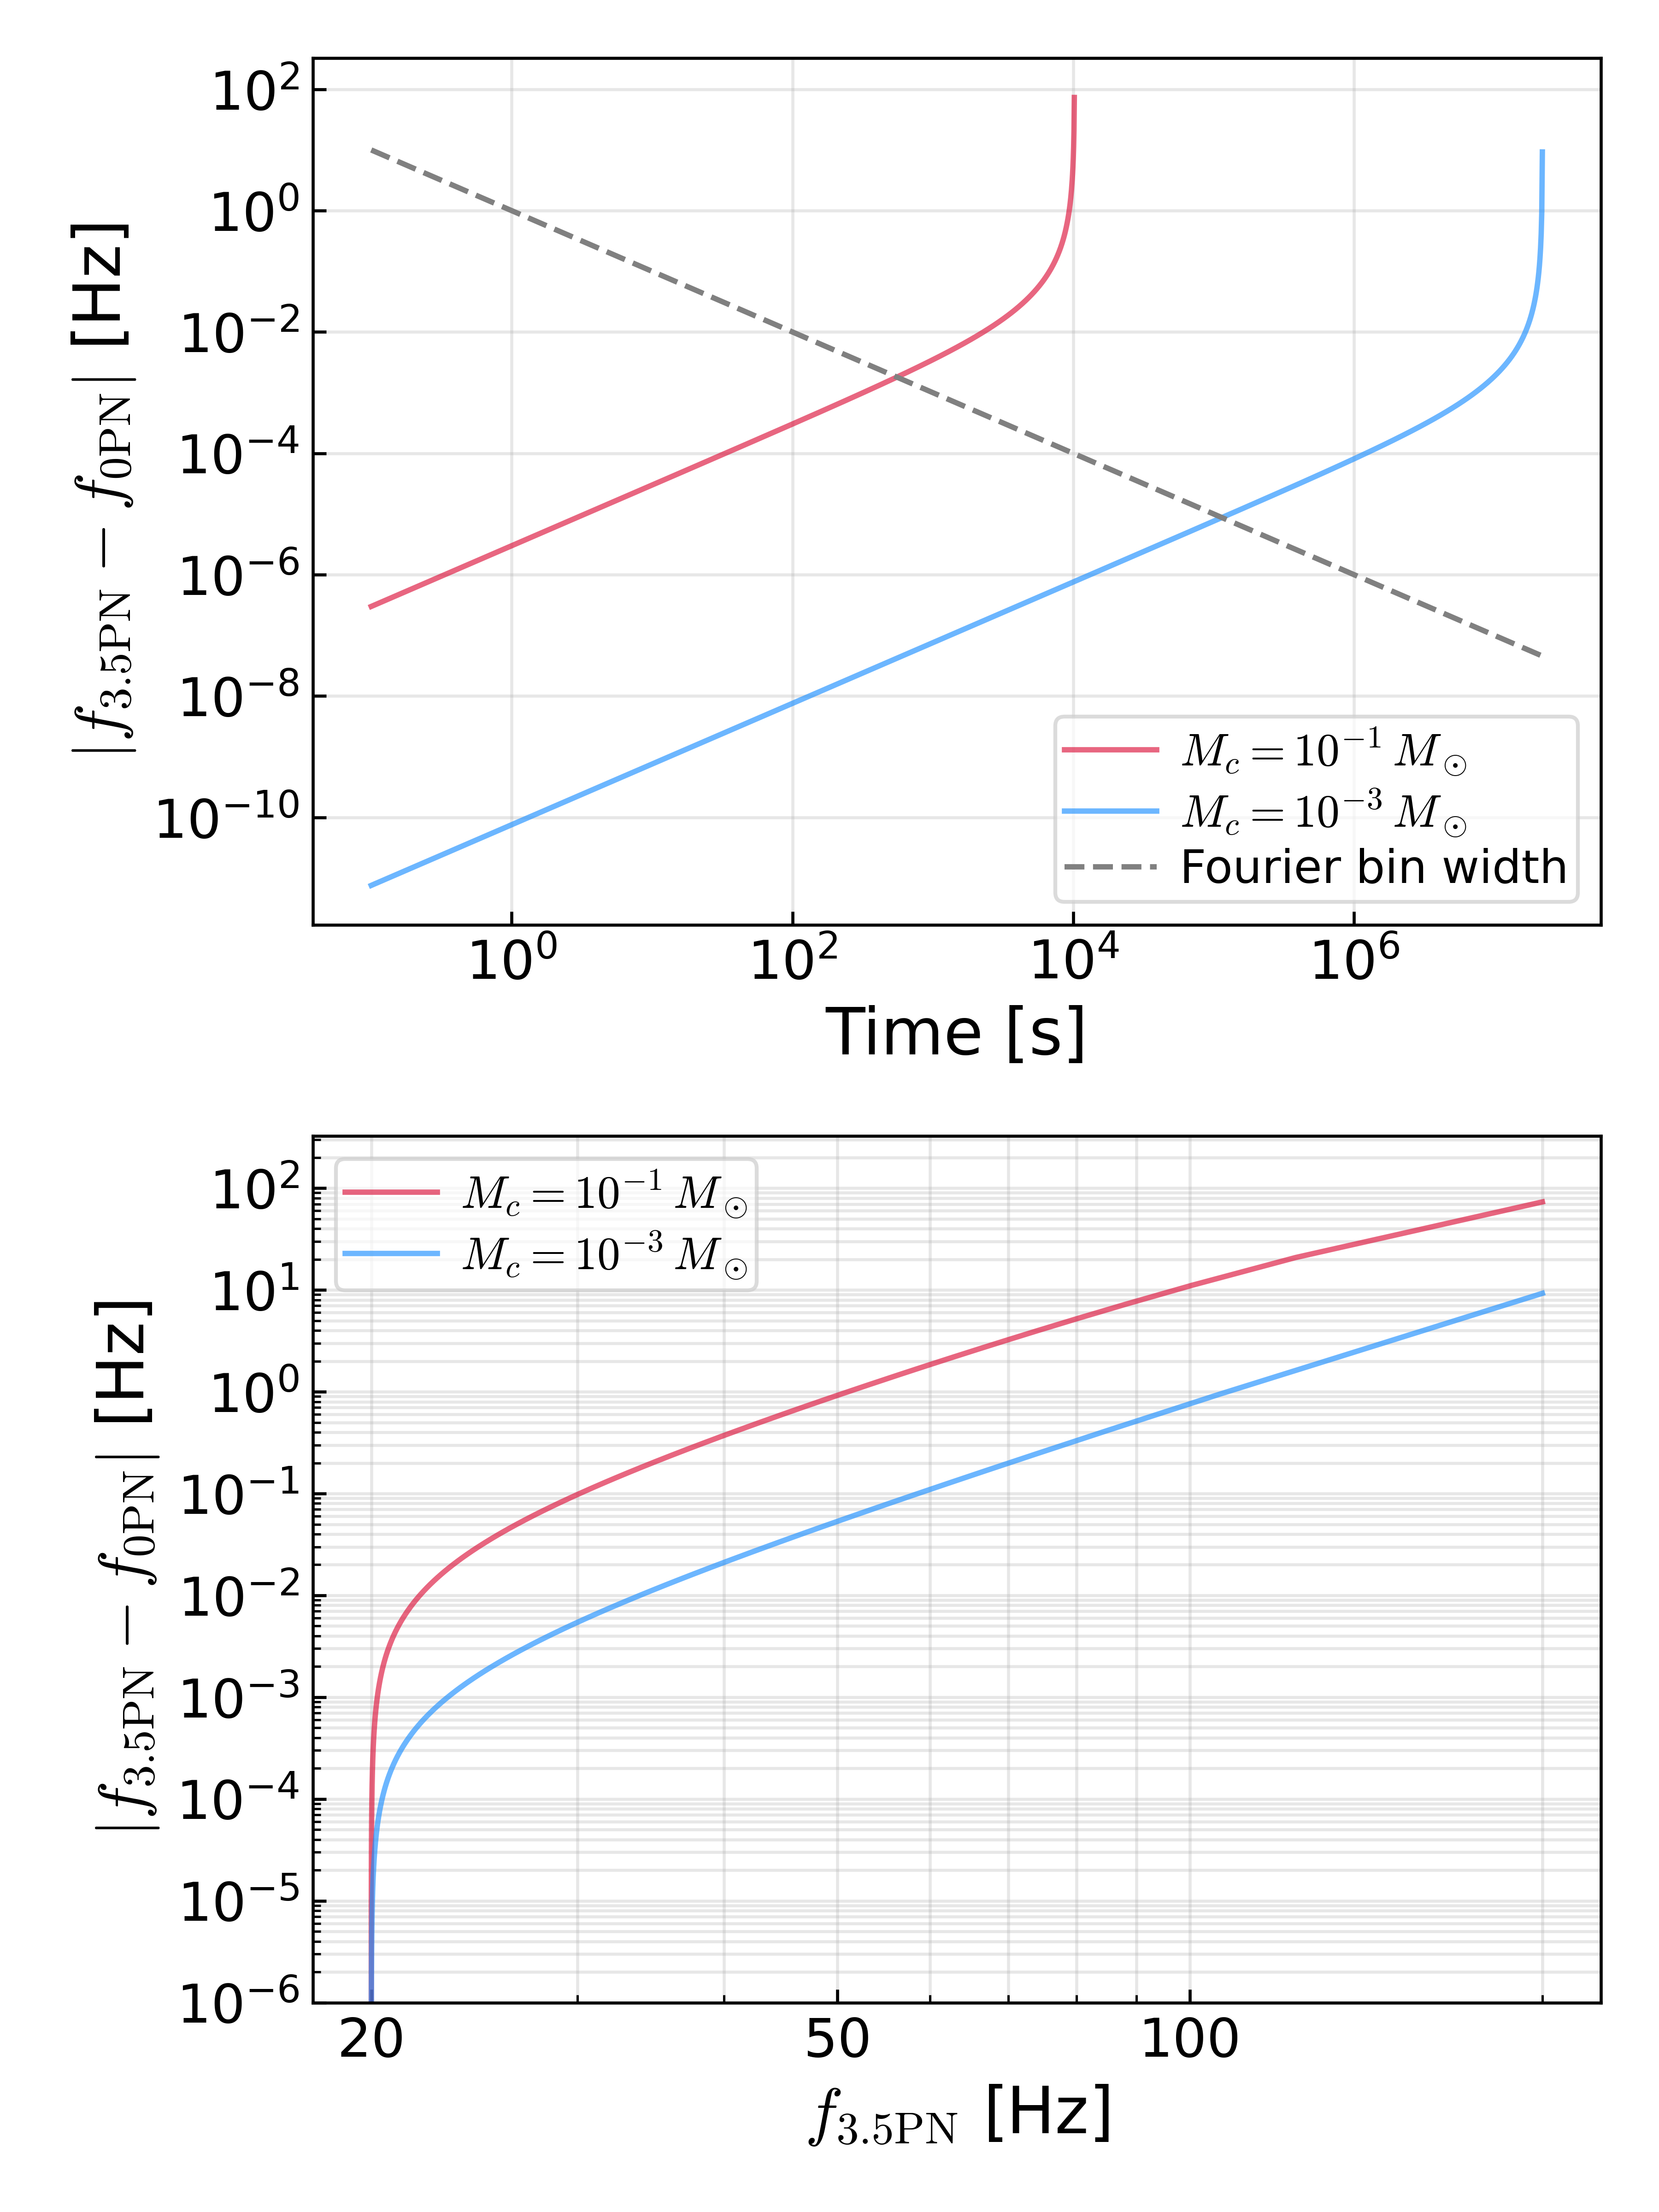
\includegraphics[width=0.95\columnwidth]{figs/PN_error.png}
\caption{
    Error between the 0PN and 3.5PN waveform models for systems with $M_c = 10^{-1}, 10^{-3}M_\odot$, $f_0 = 20$ Hz, non-spinning, equal mass-ratio. The upper (lower) panel shows the difference between the instantaneous frequencies as a function of time after a reference time (frequency of the 3.5PN model). 
}
\label{fig:PN_error}
\end{figure}

When modelling the waveform intrinsic strain amplitude, we only consider the leading order 0PN term as is common in searches for sub-solar mass binary black hole signals \cite{LIGOScientific:2026wxza, LVK:2022ydq, Kacanja:2026byy}. The intrinsic strain amplitude evolution is then: 
\begin{align}
h_0(t) &= \frac{4}{d} \left( \frac{G M_c}{c^2} \right)^{5/3} \left(  \frac{\pi f(t)}{c} \right)^{2/3}  \label{eq:h0} \\
& \simeq 1.6 \times 10^{-24} \left( \frac{d}{10 \text{kpc}}  \right) ^{-1} \\
& \quad \times\left(  \frac{M_c}{10^{-3} M_\odot} \right) ^{5/3} \left(  \frac{f(t)}{50\text{Hz}} \right)^{2/3} \, ,
\end{align}
where $d$ is the distance to the binary system. 

The strain measured by a detector is the antenna-pattern-weighted sum of the two gravitational wave polarizations,
\begin{equation}
    h(t) = F_+(t;\alpha,\delta,\psi) h_+(t) 
    + F_\times(t;\alpha,\delta,\psi) h_\times(t) ,
    \label{eq:detector_response}
\end{equation}
where $F_+$ and $F_\times$ are the detector antenna pattern functions, which depend on the source sky location $(\alpha,\delta)$, polarization angle $\psi$, and time through the rotation of the Earth. For the quadrupole harmonic:
\begin{align}
    h_+(t) &= h_0(t) \frac{1+\cos^2\iota}{2} \cos\phi(t), \\
    h_\times(t) &= h_0(t) \cos\iota \sin\phi(t),
\end{align}
where $\iota$ is the inclination of the binary orbital angular momentum relative to the line of sight and $\phi$ is the gravitational wave phase.


%==========================================================================
\section{Methods}
\label{sec:methods}
The search consists of two stages.  First, the full observing time $T_\mathrm{obs}$ is divided into segments of duration $T_{\rm coh}$. Each segment is coherently searched over using 0PN templates as described in Sec.~\ref{sec:coherent_analysis}. This coherent analysis uses a novel resampling implementation based on non-uniform fast Fourier transform (NUFFT) as detailed in Sec. \ref{sec:resampling}. The second stage of the analysis is a semicoherent combination of segments along 3.5PN frequency tracks as described in Sec.~\ref{sec:semicoherent_combination}. 

% to mitigate any finite length effects, resampled to search for a specific 0PN signal corresponding to a value of $\beta$, then Fourier transformed. This is implemented in a single step using a non-uniform fast Fourier transform (NUFFT) as detailed in Sec. \ref{sec:resampling}. This results in frequency spectra for each value of $\beta$ searched over. The second stage of the analysis is a semicoherently combination of segments along 3.5PN frequency tracks. The noise weighting of semicoherent segments must correct for the effect of NUFFT on the PSD. This analysis procedure differs from the standard peakmap used in continuous wave analysis since signal within each segment is coherently analyzed using the 0PN phase model instead of a monochromatic signal. \ls{should still be monochromatic within Tcoh after resampling}
% \ls{the descriptions here are generally too colloquial, e.g., along 3.5PN frequency tracks, correct for effect of NUFFT on the PSD; need rewording}

\subsection{Coherent analysis over $T_{\rm coh}$}
\label{sec:coherent_analysis}
The waveform in each segment is modeled using the 0PN model, which is sufficiently accurate for the short durations of each segment. We use a 0PN model instead of a Taylor expansion (as is common in other continuous wave analyses) because it better approximates the non-linear chirping structure of the 3.5PN waveform than low-order Taylor expansions. This allows longer coherent segments while retaining a low-dimensional model. At 0PN, the frequency evolution of gravitational waves emitted by a PBH binary during its inspiral can be written as:
\begin{equation}
    f_{\rm 0PN}(f_0, M_c, t) = f_0 \left( 1-\frac{8}{3}\beta(f_0, M_c) t \right)^{-3/8} \, , \label{eq:f}
\end{equation}
where $\beta$ is as defined in Eq.~\ref{eq:beta}. The corresponding phase evolution of this signal is:
\begin{equation}
    \phi_{\rm 0PN}(f_0, M_c, t) = -\frac{6\pi}{5} f_0 \frac{(1-\frac{8}{3}\beta(f_0, M_c) t)^{5/8}}{\beta(f_0, M_c)} + \phi_0 \, , \label{eq:phi}
\end{equation}
where $\phi_0$ is the phase at the reference time $t=0$. 

We select a coherent segment length such that the mismatch between the 0PN model and the full 3.5PN signal is $\mathcal{M}_{\rm PN} \leq 0.05$. We define the usual noise-weighted inner product between two waveforms $a$ and $b$ as:
\begin{equation}
(a|b)
=
4 \, {\rm Re}
\int
\frac{a^{*}(f)b(f)}{S_n(f)}\,df \, ,
\end{equation}
where $*$ is the complex conjugate and $S_n(f)$ is the one-sided noise spectral density. 
The overlap between the 3.5PN and 0PN waveforms is
\begin{equation}
\mathcal{O}(T_{\rm coh}, f_0, M_c)
=
\max
\frac{
\left(h_{\rm 3.5PN} \middle| h_{\rm 0PN}\right)
}{
\sqrt{
\left(h_{\rm 3.5PN} \middle| h_{\rm 3.5PN}\right)
\left(h_{\rm 0PN} \middle| h_{\rm 0PN}\right)
}
} ,
\end{equation}
where $h_{\rm 3.5PN}$ is a 3.5PN waveform, $h_{\rm 0PN}$ is a 0PN waveform, and relative time and phase shifts. The mismatch is defined to be:
\begin{equation}
\mathcal{M}_{\rm PN}(T_{\rm coh}, f_0, M_c)
=
1 - \mathcal{O}(T_{\rm coh}, f_0, M_c).
\end{equation}
We require
\begin{equation}
\max_{f_0,M_c}
\mathcal{M}_{\rm PN}(T_{\rm coh}, f_0, M_c)
= 0.05 = \mathcal{M}_{\rm max}
\label{eq:coherent_mismatch_max}
\end{equation}
for the parameter space considered this enforces a maximum coherence time of $32$~s, so we choose $T_{\rm coh}=30~{\rm s}$. It also possible to choose different coherence times when analyzing different regions of the parameter space, but we leave this for future work. 

When analyzing signals, we need to search over $\beta$, which is not known a-priori. To do this we build a template bank over $\beta$ which varies between $3\times10^{-8} \lesssim \beta  \lesssim 7\times10^{-4}$. We construct the template bank such that the mismatch between the $h_{\rm 3.5PN}$ and the closest 0PN template is less than the mismatch criterion we set earlier $\mathcal{M}_{\rm PN} \ 0.05$. We compute this numerically and uniformly placing templates in $\beta$ such that the mismatch condition is satisfied for the full parameter space. We require 69 templates to span the full $\beta$ range considered. 

%==========================================================================
\subsection{Resampling with non-uniform fast Fourier transforms}
\label{sec:resampling}
Within each coherent segment, we search for the 0PN templates using resampling. Resampling is a signal-processing technique used to remove the expected phase evolution of a signal by changing the time coordinate in which the data is sampled. Data which matches the template will then be monochromatic and matched filtering is performed using a Fast Fourier Transform (FFT) operation. Resampling was originally proposed for gravitational wave signals in \cite{Smith:1987hh} and specifically for continuous gravitational waves in \cite{livasBroadbandSearchTechniques1989, Jaranowski:1998qm, Astone:2010ct, Braccini:2011zz}. More recent implementations are described in \cite{Astone:2014dea, Mastrogiovanni:2017xjr, Meadors:2017pefa, Singhal:2019dfn}, and used in observational searches described in \cite{LIGOScientific:2026qsb, LIGOScientific:2017ytx}. 

The basic idea of resampling is to define a new time variable with respect to which the signal is monochromatic. For PBH binaries, we define the new time variable:
\begin{equation}
\tau(\beta) = -\frac{3}{5} \frac{(1-\frac{8}{3}\beta t)^{5/8}}{\beta} , \label{eq:new_t}
\end{equation}
Substituting Eq. \ref{eq:new_t} into Eq. \ref{eq:phi} gives:
\begin{equation}
\phi_{\rm 0PN}(\beta, \tau) = 2\pi f_0 \tau(\beta) + \phi_0,\label{eq:monochromatic}
\end{equation}
i.e. the signal is monochromatic with respect to $\tau$. A demonstration of the basic principle of resampling is shown in Fig. \ref{fig:resampling_picture} where a signal with an evolving frequency is resampled and is monochromatic with respect to the resampled time coordinate. For fixed values of the remaining signal parameters, the unknown reference frequency $f_0$ appears simply as the Fourier frequency in the resampled time coordinate. Consequently, the Fourier amplitude in each frequency bin is proportional to the matched-filter output for the template with the corresponding value of ($f_0$). A single FFT therefore evaluates a bank of templates spanning many reference frequencies simultaneously, rather than requiring each template to be computed separately. This is shown in Fig.~\ref{fig:resampling_spectra} which shows a signal with an evolving frequency whose signal power is spread over many Fourier bins. After resampling, the signal power is concentrated in a single Fourier bin. 
%, but it is more robust in the presence of data gaps, which are likely to be present when searching for long-lived signals. \nl{Maybe too risky to say}

\begin{figure}
\centering
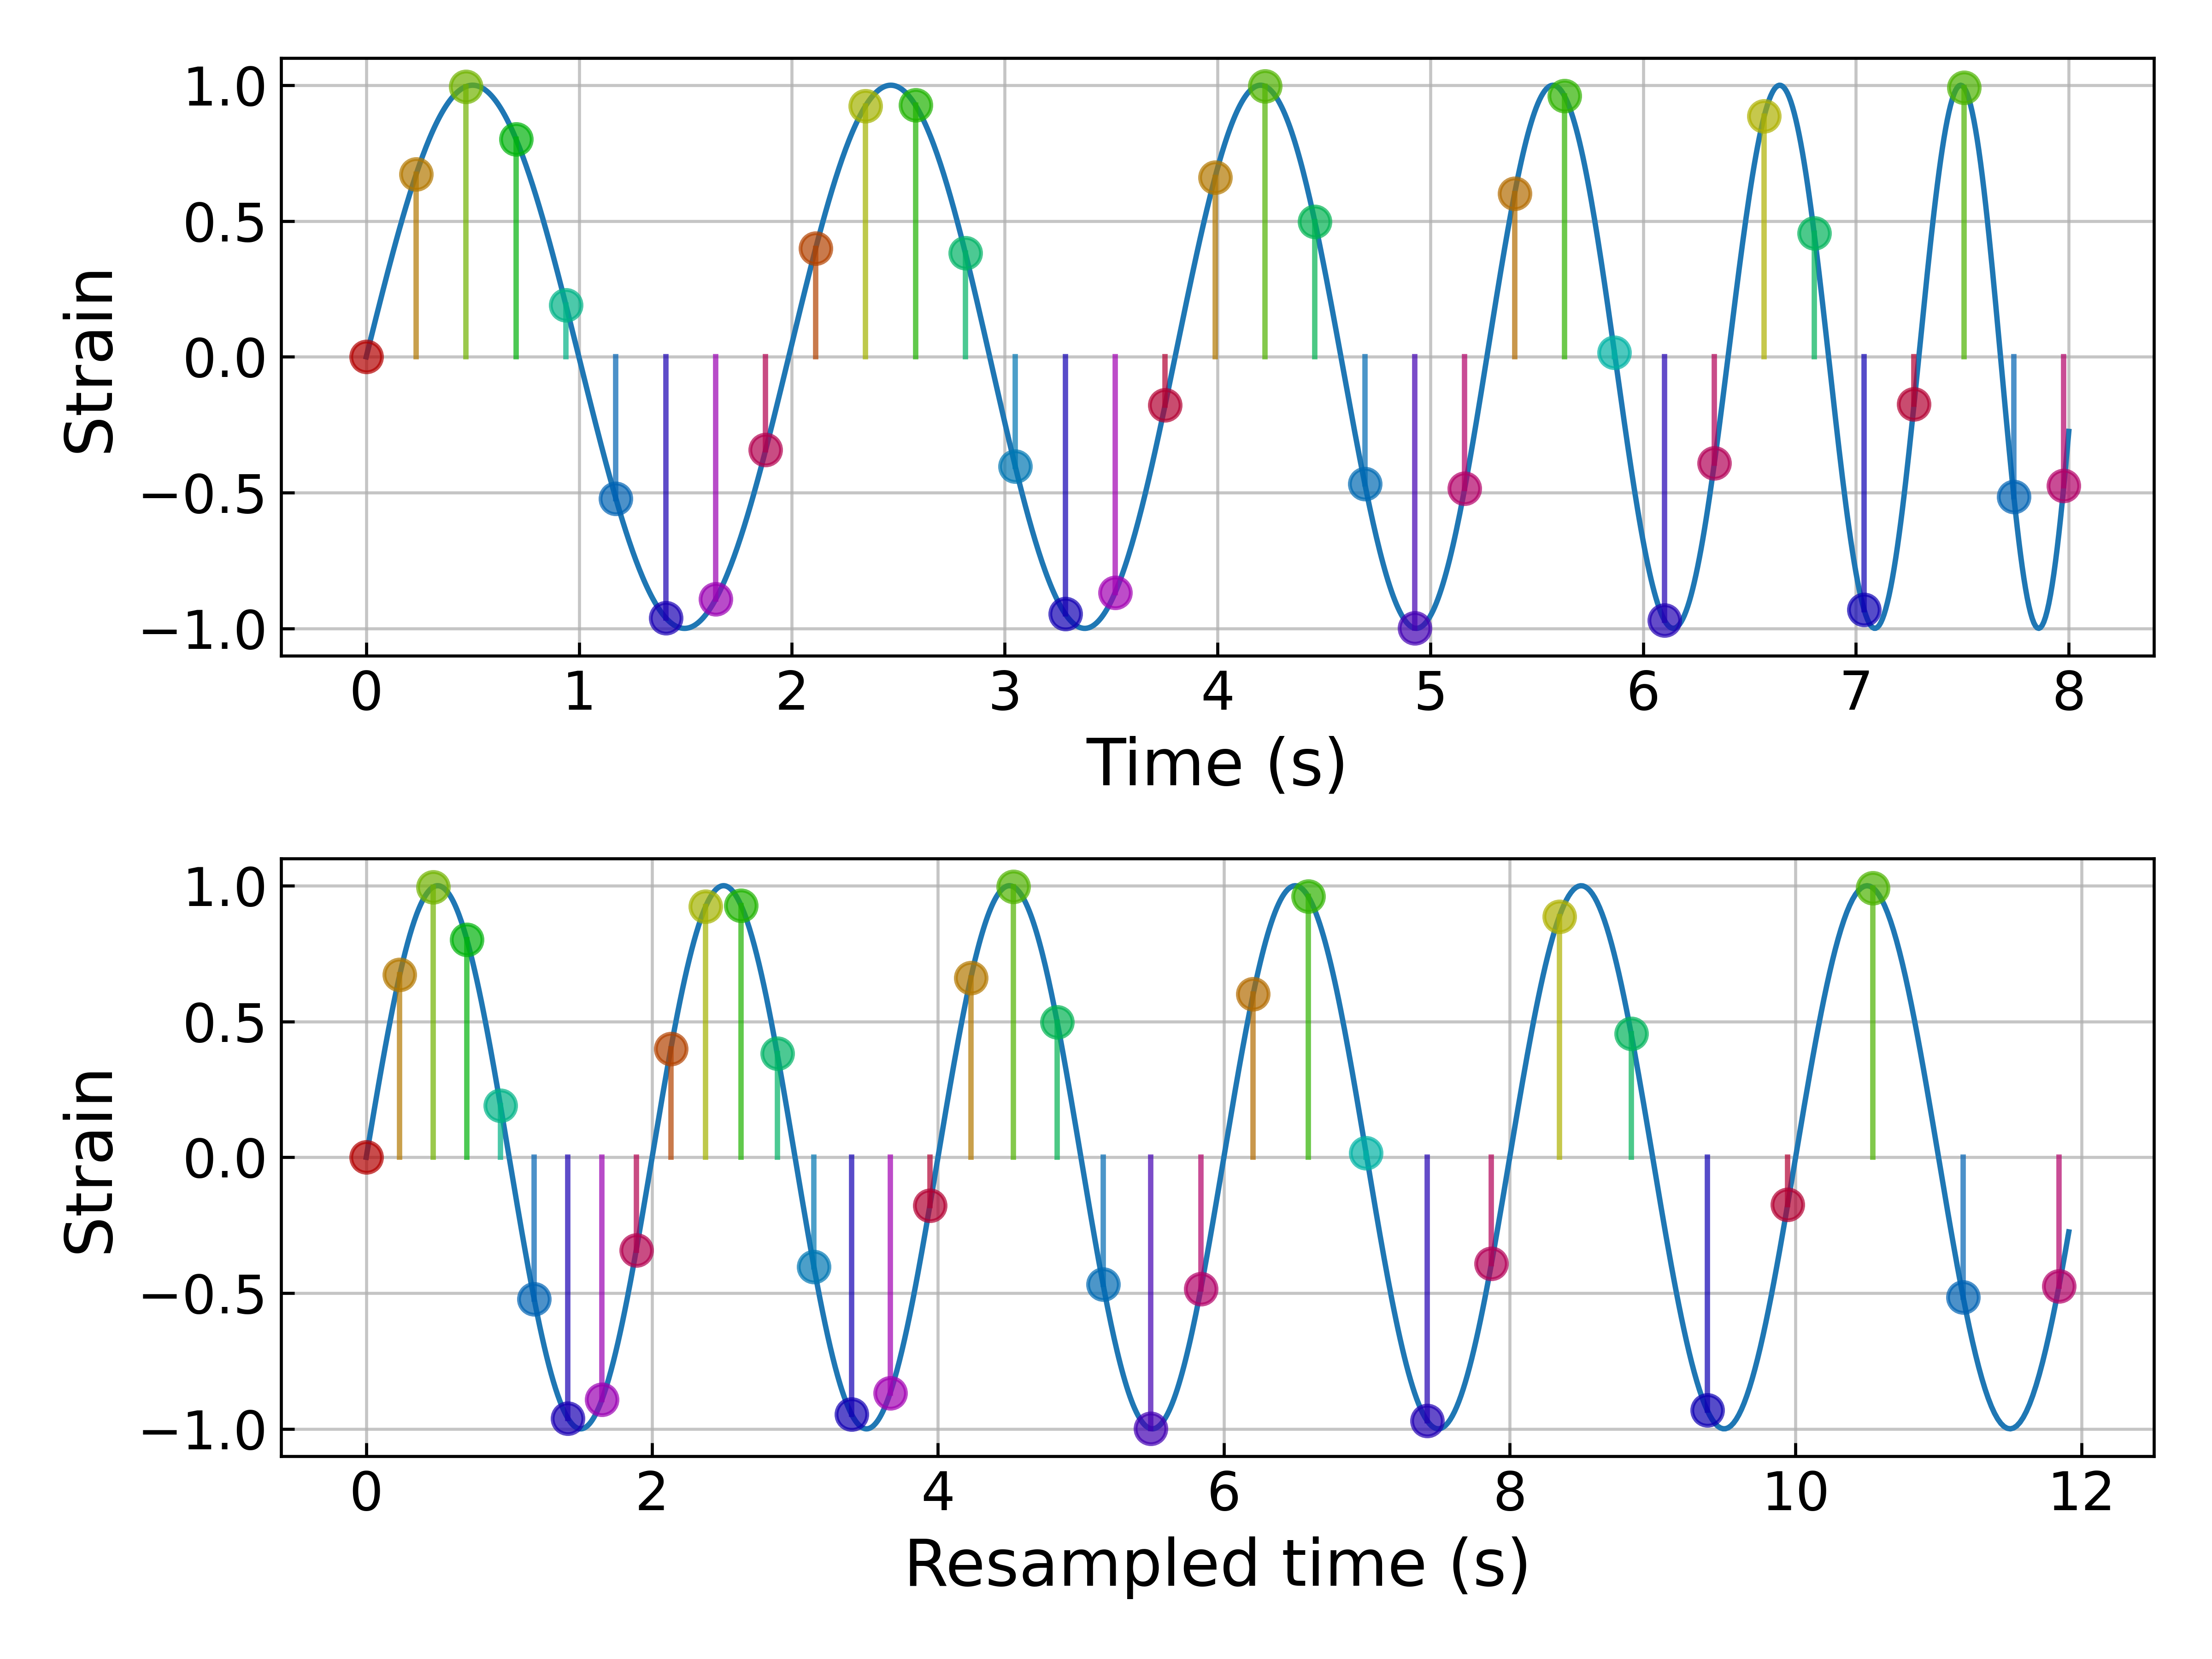
\includegraphics[width=0.95\columnwidth]{figs/resampling_graphic.png}
\caption{
Resampling transforms a chirping, uniformly sampled signal into a monochromatic, non-uniformly sampled time series. The colors correspond to the signal phase and show the same data points are used even after the signal is resampled.
}
\label{fig:resampling_picture}
\end{figure}

\begin{figure}
\centering
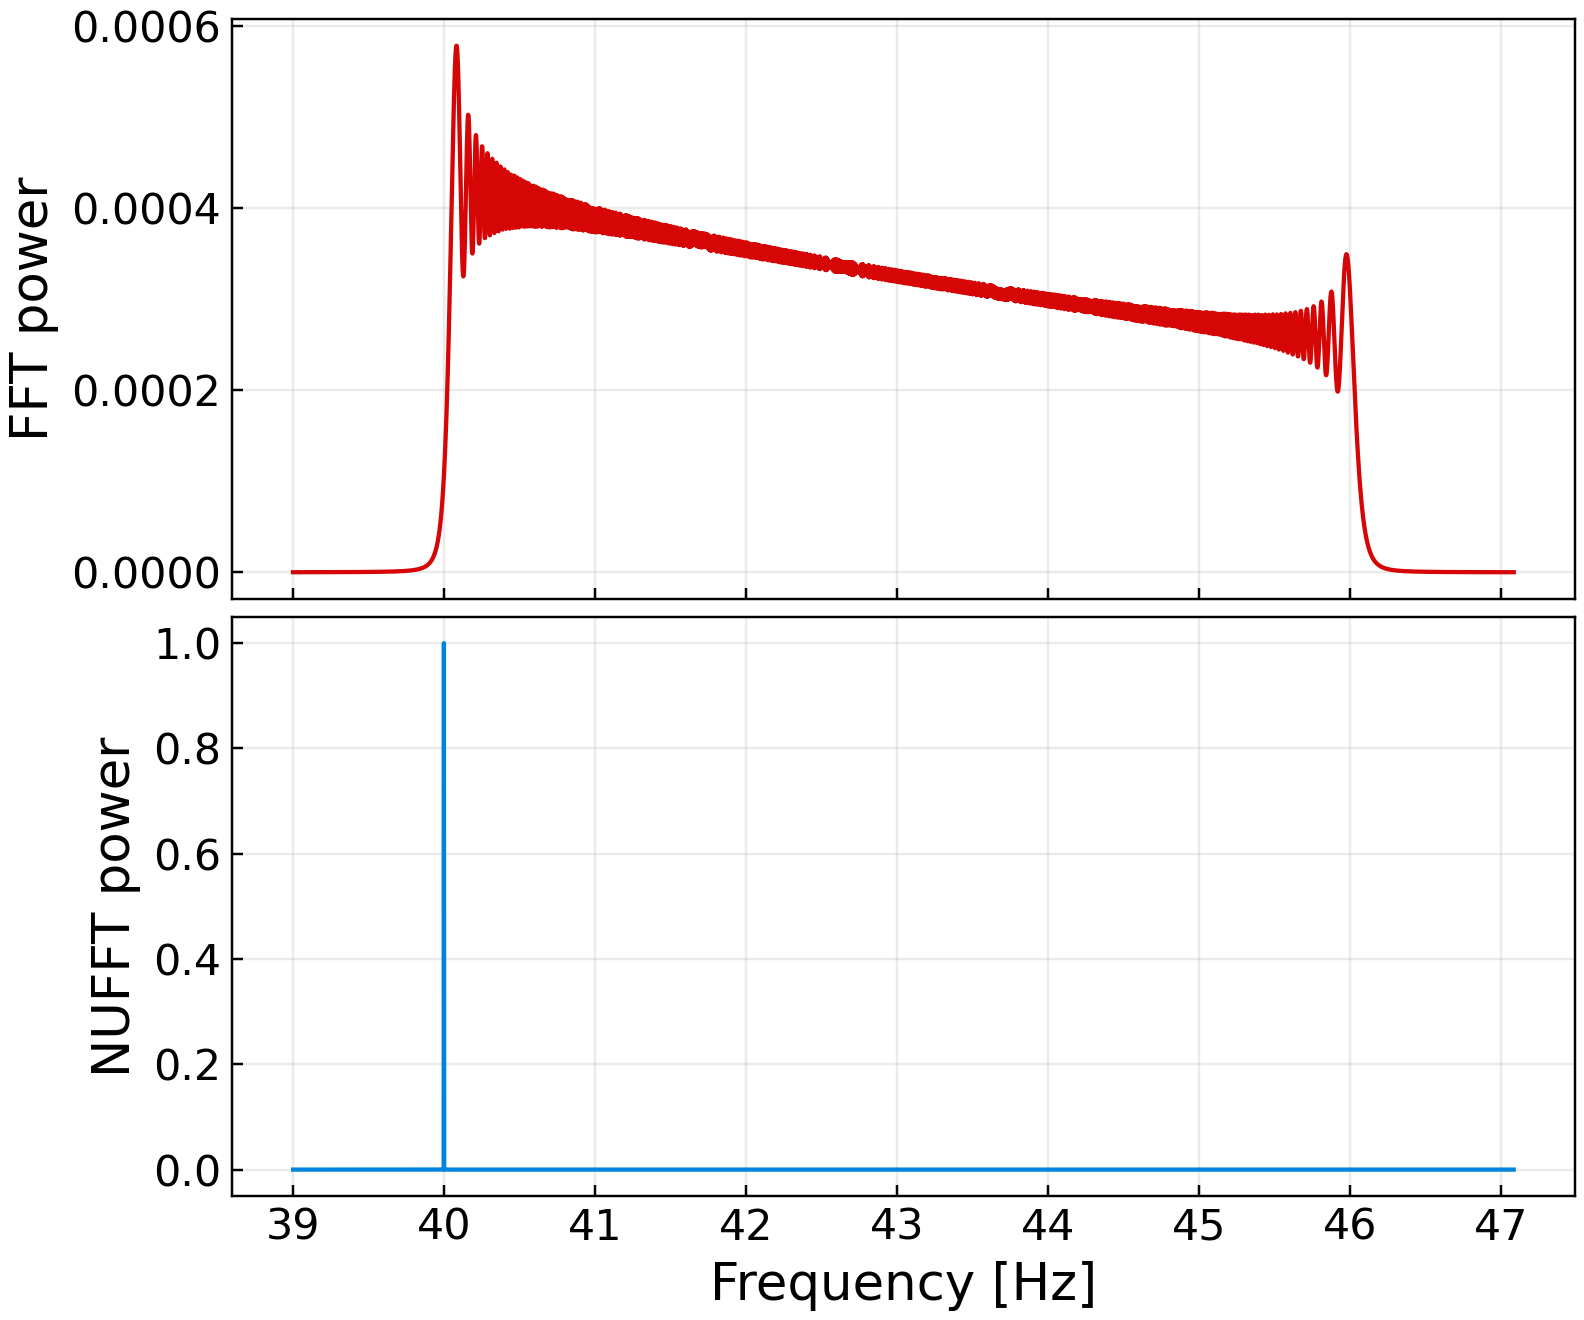
\includegraphics[width=0.95\columnwidth]{figs/resampling_example.png}
\caption{
Resampling transforms a chirping signal with an evolving frequency to a monochromatic signal whose signal power is confined within a single Fourier bin. 
}
\label{fig:resampling_spectra}
\end{figure}

However, after resampling, the signal is not uniformly sampled with respect to the new time variable $\tau$ and so cannot be directly FFTed. Different resampling implementations use different techniques to effectively interpolate the signal onto a uniform time grid in the resampled time so that it can be Fourier transformed. Previous implementations of resampling used "stroboscopic" resampling \cite{Jaranowski:1998qm, Astone:2010ct, Singhal:2019dfn}, where a higher sampling frequency is used for the original time series and nearest-neighbour interpolation is used to create a resampled time series that is uniformly sampled. However, nearest-neighbour interpolation is equivalent to convolution with a rectangular kernel and can introduce aliasing and errors in the resampled FFT unless the original time series is sampled at a higher rate and subsequently downsampled when computing the FFT. This oversampling requirement increases the computational cost of stroboscopic resampling. We provide a brief explanation in Appendix~\ref{sec:resampling_convolution} of how different resampling methods correspond to difference choices of convolution kernel.

Computationally cheaper implementations of resampling use different choices of kernel function when interpolating the resampled timeseries onto a uniform time grid. We are ultimately interested in the Fourier transform of the resampled timeseries, rather than the timeseries itself, for which there is a relevant body of work in applied mathematics on computationally efficient choices of kernels. The operation of interpolating and Fourier transforming is known as a type-I NUFFT \cite{duttFastFourierTransforms1993, Barnett:2019FINUFFT}. There are many NUFFT methods and implementations corresponding to different choices of kernel function. For older review articles with accessible introductions to the subject, see \cite{greengardAcceleratingNonuniformFast2004, wareFastApproximateFourier1998}. For modern implementations on CPUs and GPUs see \cite{finufftFlatironinstituteFinufftNonuniform, shihCuFINUFFTLoadbalancedGPU2021, linJyhmiinlinPynufft2023, vaillantGhisvailPyNFFT2023, vanderplasJakevdpNfft2023, ouGNUFFTWAutoTuningHighPerformance2017} and the references within. Throughout the rest of this work we use the fiNUFFT implementation described in \cite{2019SJSC...41C.479B}. 

The speedup between NUFFT and stroboscopic resampling as a function of the desired resampling accuracy is benchmarked using 4 threads on a commercial Intel 255U CPU and results shown in Fig. \ref{fig:NUFFT_speedup}. It shows the significant speedups can be achieved by using NUFFT implementations. Some stroboscopic resampling implementations in continuous wave searches use parameters corresponding to an accuracy of $\approx 0.025$. This benchmarking shows speedups of $\mathcal{O}(10)$ could be achieved but should be taken only as an indicative value since actual speedups will depend on coherence length, CPU model, and numerical implementations. 

\begin{figure}
\centering
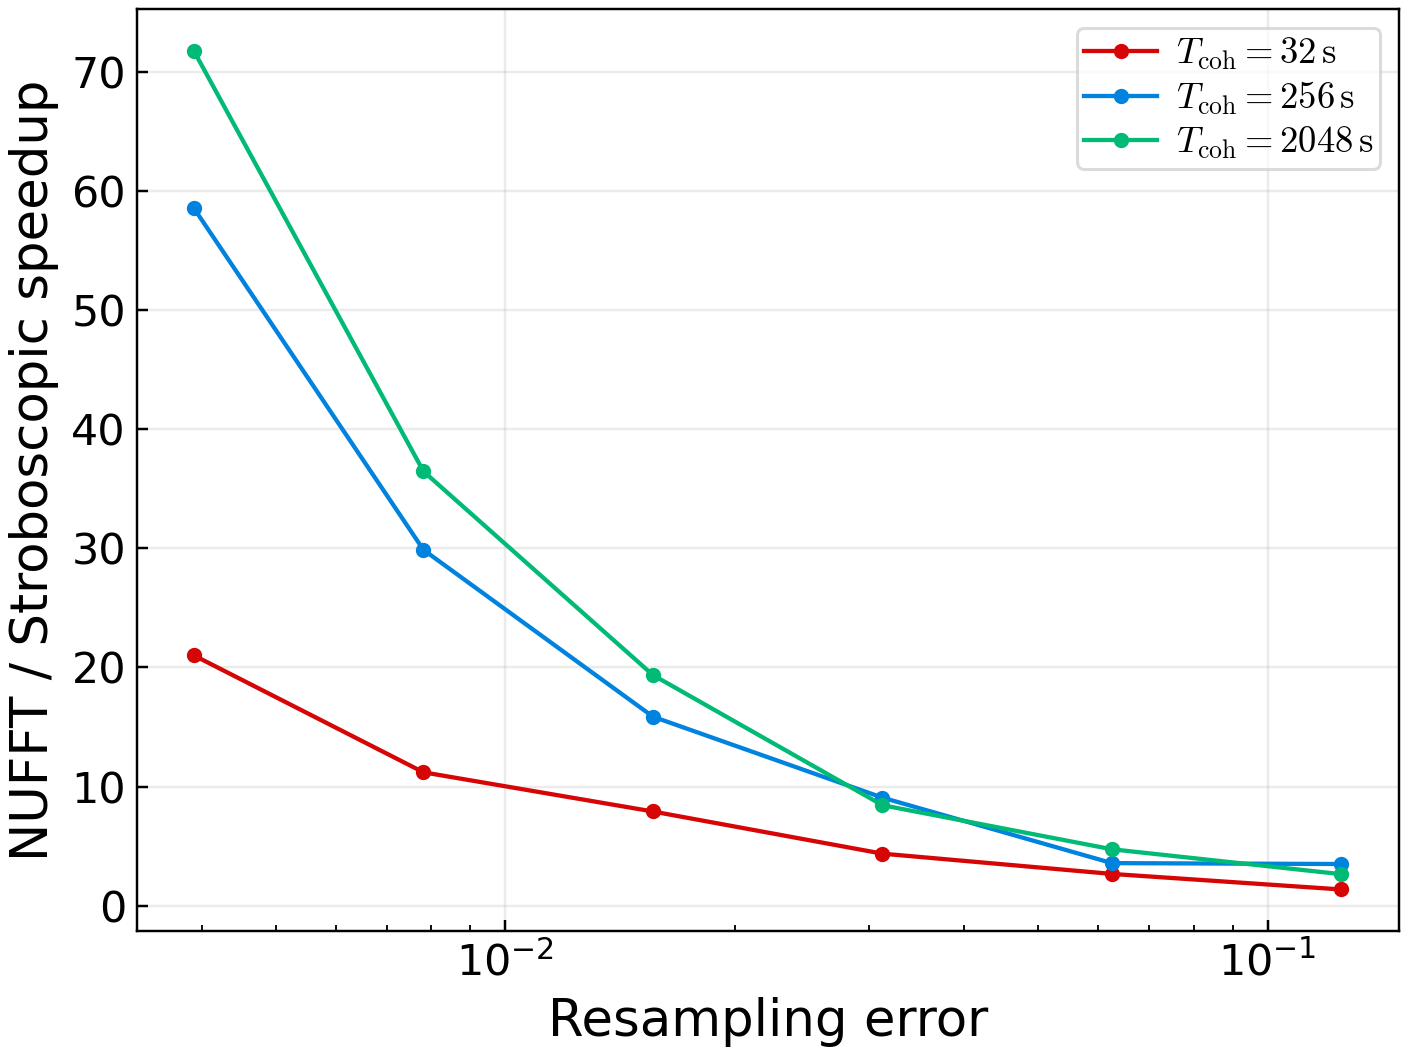
\includegraphics[width=0.95\columnwidth]{figs/2d_strobo_vs_nufft_speedup.png}
\caption{
Speedup of using NUFFT compared to stroboscopic resampling as a function of resampling error for $f_0 = 20,\mathrm{Hz}$, $M_c = 10^{-2} M_\odot$, $f_\mathrm{sampling} = 512 \, \mathrm{Hz}$ and $T_\text{obs} = 32, 256, 2048 \,\mathrm{s}$. 
}
\label{fig:NUFFT_speedup}
\end{figure}

\subsection{Semicoherent combination over $T_{\rm obs}$}
\label{sec:semicoherent_combination}
After the coherent analysis using resampling, the data are represented by a collection of resampled spectra indexed by resampled Fourier frequency $f$, segment start time $t_i$, and $\beta$. These spectra may then be combined along the frequency evolution of a candidate signal using any suitable semicoherent method, including peakmaps \cite{Astone:2014esa, Miller:2018rbg, Piccinni:2018akm}, Hough-transform \cite{Krishnan:2004sv, Astone:2014esa, Mendell_stackslide_hough, Miller:2018rbg}, $\mathcal{F}$-statistic \cite{Jaranowski:1998qm}, or Viterbi-based approaches \cite{Suvorova:2016rdc, Sun:2017zge, Alestas:2024ubs}. Note that these methods would need to be modified to operate on higher dimensional tracks since our spectra are three dimensional $\{f, t_i, \beta\}$ rather than the usual two dimensional time-frequency maps. In this work, we describe a noise-weighted stack-slide implementation \cite{Brady:1998nj, Mendell_stackslide_hough}. 

The stack-slide method accumulates the power along a frequency template. The parameters of the semicoherent frequency template are $\theta=\{M_c, t_{\rm ref}\}$ where $t_{\rm ref}$ is the reference time when the template enters the analysis band which is fixed a-priori. In the $i$-th segment, this model corresponds to a Fourier frequency $f_i(\theta)$ and 0PN resampling template $\beta_i(\theta)$ which was used for the coherent analysis within the segment. Let $C(\theta)$ be the set of segments for which the template frequencies are within the analysis band such that $N_{\rm seg}(\theta) = |C(\theta)|$. 

For a given segment, we define the normalized power as:
\begin{equation}
P_i(\theta)
=
\frac{4\left|\widetilde{x}_i\left[f_i(\theta), \beta_i(\theta)\right]\right|^2}
{T_{\rm coh} S_i^{\rm eff}\left[f_i(\theta), \beta_i(\theta)\right]},
\label{eq:normalized_power}
\end{equation}
where $\widetilde{x}_i(f, \beta)$ is the Fourier amplitude of the $i$-th segment after resampling with $\beta$, and $S_i^{\rm eff}(f, \beta)$ is the effective one-sided noise PSD after accounting for the effects of resampling and windowing. 

The relative weight of segment $i$ is:
\begin{equation}
w_i(\theta)
\propto
\frac{A_i^2(\theta)\Gamma_i}
{S_i^{\rm eff}\left[f_i(\theta), \beta_i(\theta)\right]}, \label{eq:weights}
\end{equation}
where $A_i^2(\theta)$ is the average squared signal amplitude and $\Gamma_i$ accounts for
the windowing function. The weights are normalized to satisfy: 
\begin{gather}
    \sum_{i \in C(\theta)}w_i^2(\theta)=1 .
\end{gather}
The short coherent times mean that the search can apply omni-directionally without specifying a sky location, and in this case $A_i^2(\theta)$ depends only on the intrinsic signal parameters. It, however, also possible to target the search to a particular sky-location and account for a particular detector antenna response functions $F_{+/\times}(t;\alpha,\delta,\psi)$ in the weighting function, leading to gains in sensitivity that will be demonstrated shortly.

The semicoherent statistic is then:
\begin{equation}
n_\sigma(\theta)
=
\sum_{i\in C(\theta)}
w_i(\theta)
\frac{P_i\left[f_i(\theta)\right]-\mu_i}{\sigma_i}
,
\label{eq:semicoherent_statistic}
\end{equation}
where $\mu_i$ and $\sigma_i$ are the mean and standard deviation of $P_i$ for the background. For stationary Gaussian noise, $P_i$ is distributed according to a $\chi_2^2$ distribution and $\mu_i=2$ and $\sigma_i=2$, but for detector noise they can be computed empirically. 

Under the null hypothesis $H_0$, $n_\sigma$ has zero mean and unit variance. For equal weights, its distribution is an affine transformation of a $\chi_{2N_{\rm seg}}^2$ distribution. For unequal weights we can evaluate its distribution and survival function numerically. Given a false-alarm probability FAP, we define the detection threshold $n_\sigma^{\rm thresh}$ such that:
\begin{gather}
    p(n_\sigma > n_\sigma^{\rm thresh} | H_0) = {\rm FAP} .
\end{gather}
Fig.~\ref{fig:chi2_threshold} shows how the weighting changes $n_\sigma^{\rm thresh}$ compared to the equally weighted case for signals with initial frequency of $f_0=40$~Hz and chirp masses of $M_c = 10^{-1}, 10^{-2}M_\odot$. The weighted $n_\sigma^{\rm thresh}$ is larger by $5\%, 0.7\%, 0.1\%$ for $M_c = 10^{-1}, 10^{-2}, 10^{-3}$ ($10^{-2}$) $M_\odot$ respectively. For the majority of the parameter space the $n_\sigma^{\rm thresh}$ computed assuming uniform weights is a close approximation of the weighted threshold. 

\begin{figure}
\centering

\includegraphics[width=0.95\columnwidth]{figs/weighted_chi2_threshold.png}
\caption{
$n_\sigma^{\rm thresh}$ as a function of false-alarm probability for the weighted and unweighted $\chi^2_{2M}$ distributions. The weights used are for signals with initial frequency of $f_0=40$~Hz and chirp masses of $M_c = 10^{-1}, 10^{-2}, 10^{-3}$. 
}
\label{fig:chi2_threshold}
\end{figure}

In the presence of a signal $H_\theta$, $P_i$ is distributed according to a non-central $\chi_2^2$ distribution with $\mu_i=2+\lambda$, where $\lambda$ is the non-centrality parameter and equal to the normalized power (defined in Eq.~\ref{eq:normalized_power}) of the signal in the particular segment. In this case, $n_\sigma$ is an affine transformation of a weighted, non-central $\chi_{2N_{\rm seg}}^2$ distribution with non-centrality $\Lambda=\sum_{i\in C(\theta)} w_i(\theta)\lambda(\theta)$. Weighting different segments is crucial for PBH signals as they chirp large frequency ranges such that the signal amplitude and PSD can vary significantly. Accounting for the weights can increase the recovered $n_\sigma$ up to $20\%$ for PBH signals in this parameter range. 

The improvement in signal detectability is shown using a receiver operating characteristic (ROC) curve in Fig.~\ref{fig:roc} which plots the true-positive probability (TPP) against the FAP. We inject signals with randomised sky-locations and analyze them without any noise. We compute the TPP as the fraction of injected signals which exceeded $n_\sigma^{\rm thresh}$. The all-sky search, where the antenna-responses are marginalized over but the intrinsic amplitude evolution is accounted for, leads to a small improvement in sensitivity compared to the unweighted search. Targeting a particular sky-location, however, markedly increases the detectability of the signal and demonstrates the improved sensitivity of targeted searches even though the short coherence lengths of the search allow for all-sky searches. 

\begin{figure}
\centering

\includegraphics[width=0.95\columnwidth]{figs/weighted_vs_equal_roc.png}
\caption{
ROC curve for signals with $M_c = 10^{-3}M_\odot$, $f_0=40$~Hz, $f_{\rm high}=60$~Hz with randomized sky-locations and $d=50$~kpc. Demonstrates that accounting for the signal weights improves detectability, especially when targeting a specific sky-location. 
}
\label{fig:roc}
\end{figure}

This semicoherent stage requires a bank of 3.5PN templates distinct from the 0PN $\beta$ templates used for each coherent segment. We define the semicoherent mismatch as:
\begin{equation}
    \mu(\theta, \theta_s) = 1-\frac{n_\sigma(\theta|\theta_s)}{n_\sigma(\theta_s|\theta_s)} \, , \label{eq:semicoherent_mismatch}
\end{equation}
where $n_\sigma(\theta|\theta_s)$ is the semicoherent statistic for a template $\theta$ given the presence of a signal with true parameters $\theta_s$ without the presence of noise. We require:
\begin{equation}
    \max_{\theta, \theta_s}\mu(\theta, \theta_s) = 0.05 = \mu_{\rm max} \label{eq:semicoherent_mismatch_max}
\end{equation}

We estimate the required size of the template bank using a geometric approach, standard in semicoherent searches \cite{Prix:2007ks,Wette:2014tca}. Other algorithms developed for
compact-binary template banks \cite{Brown:2012nn}, including
MANIFOLD-style, stochastic, or hybrid bank-generation strategies
\cite{Hanna:2022zpk,Hanna:2024tom,Kacanja:2024pjh,Roy:2017oul,Roy:2017qgg},
could be adapted to the semicoherent mismatch and applied.  Such algorithms may
produce smaller banks at fixed retained power, particularly near boundaries or
in regions where the local metric varies rapidly. 

In the geometric approach we define a metric:
\begin{equation}
g_{ab}(\theta_s)
=
-\frac{1}{2n_\sigma(\theta_s;\theta_s)}
\left.
\frac{\partial^2 n_\sigma(\theta;\theta_s)}
{\partial\theta^a\partial\theta^b}
\right|_{\theta=\theta_s} ,
\label{eq:semicoherent_metric_tensor}
\end{equation}
and use this to approximate Eq. \ref{eq:semicoherent_mismatch} at a small offset $\Delta\theta$ from the true signal parameter $\theta_s$ using a quadratic form: 
\begin{align}
\mu(\theta_s+\Delta\theta;\theta_s;)
&\simeq  g_{ab}(\theta_s)\Delta\theta_a\Delta\theta_b
\label{eq:semicoherent_metric_expansion}
\end{align}
with implicit summation over $a, b$. Here we numerically differentiate the TaylorF2
signal model to obtain the non-uniform metric. 

We use the metric to compute the number of templates required:
\begin{equation}
    N \simeq \Theta
    {\mu_{\max}}^{-n/2}
    \int_{\rm bank}
    \sqrt{\det g(\theta)}
    \,dM_c\,dt_{\rm ref}.
    \label{eq:standard_template_count}
\end{equation}
where $n$ is the dimension of the bank and $\Theta$ is the dimensionless
covering factor set by the lattice geometry.  In two dimensions,
$\Theta=1/2$ for a square covering and
$\Theta=2/(3\sqrt{3})$ for a hexagonal covering \cite{Jaranowski:2005hz}. For a hexagonal covering, this gives
an estimate of $2\times 10^{10}$ templates required. 

\section{Distance sensitivity}
\label{sec:distance_sens}
In this section, we compute the horizon distance for this semicoherent search using the O4 design sensitivty ASD, find the dependence of this on the choice of analysis frequency band, and justify our choice of analyzing signals between 40--60 Hz. We define the horizon distance as the distance at which a signal is
detected with probability $p_{\rm det}$ with a noise-only
false-alarm probability FAP. The threshold noncentrality $\Lambda_{N_{\rm seg}}^{\rm thresh}$ required to obtain 
$p_{\rm det}$ at the chosen FAP when $N_{\rm seg}$ segments
are combined is defined such that:
\begin{equation}
    p\!\left(
        n_\sigma>n_\sigma^{\rm thresh}
        \mid \Lambda=\Lambda_{N_{\rm seg}}^{\rm thresh}
    \right)
    =p_{\rm det}. 
    \label{eq:noncentrality_threshold}
\end{equation}
We first consider a
fully coherent analysis over the in-band signal duration and choose ${\rm FAP}=10^{-6}$ and ${\rm FAP}=0.95$ and find $\Lambda_1^{\rm thresh}=46.5$. After averaging over sky position,
inclination, polarization, and Fourier-bin offset, the coherent (matched filter) distance
sensitivity is:
\begin{align}
  d_{\rm coh}(M_c,f_0,f_{\rm high}) =& 
  \frac{0.007517 \, c \, \beta(f_0,M_c)}
  {f_0^{8/3} \left(\Lambda_1^{\rm thresh}\right)^{1/2}} \nonumber\\
  \times& \left(\int_{t(f_0)}^{t(f_{\rm high})}
  \frac{f(f_0,M_c, t)^{4/3}}
  {S_n[f(t,M_c)]}dt\right)^{1/2}
\end{align}
where $f_{\rm 3.5 PN}(f_0,M_c, t)$ is the 3.5PN TaylorF2 frequency track, $f_{\rm high}$ is the upper limit of the analysis frequency band, and $t(f)$ is the time when the signal reaches a signal $f$. We define the lower limit of the frequency band as $f_{\rm low}=\min(f_0)$. Here and throughout this section, we make the simplifying assumption that the signal enters and exits the analysis band within the observing time. This is reasonable because many of the signals considered have in-band durations of less than one year, which we take to be the typical duration of a gravitational-wave observing run.

The semicoherent distance sensitivity represents a computationally feasible search which accounts for the mismatches due to the coherent power loss
$\mathcal{M}{\rm max}=0.05$, semicoherent-bank power loss $\mu_{\rm max}=0.05$, and lower sensitivity inherent to semicoherent analysis which is given by:
\begin{equation}
    \mathcal{P}_{N_{\rm seg}}
    \equiv
    \left(
        \frac{\Lambda_1^{\rm thresh}}
             {\Lambda_{N_{\rm seg}}^{\rm thresh}}
    \right)^{1/2}
    \propto N_{\rm seg}^{-1/4}
    \quad (N_{\rm seg}\gg1).
    \label{eq:semicoherent_penalty}
\end{equation}
Note that $\mathcal{P}_{N_{\rm seg}}$ implicitly depends on $f_{\rm low}$ and $f_{\rm high}$ (which controls $N_{\rm seg}$) and we recover the standard $N_{\rm seg}^{-1/4}$ scaling in the limit of a large number of segments. The semicoherent horizon distance is then:
\begin{equation}
\begin{aligned}
    d_{\rm semi}(M_c,f_0,f_{\rm high})
    &= \mathcal{P}_{N_{\rm seg}}(1-\mu_{\rm max})(1-\mathcal{M}_{\rm max})^{1/2} \\
    &\quad \times 
         d_{\rm coh}(M_c,f_0,f_{\rm high}).
\end{aligned}
    \label{eq:semicoherent_dist_sens}
\end{equation}
Fig.~\ref{fig:semicoherent_sensitivity_1d} plots $\max_{f_0 \in [f_{\rm low}, f_{\rm high}]} d_{\rm semi}$ for three representative choices of analysis frequency band. In these computations we use equal weight calculation to compute this penalty from semicoherent analysis which is a sufficiently close approximation to the penalty from unequal weights because we are interested in an order of magnitude distance sensitivity. Different choices lead to different $T_{\rm coh}$ for the coherent segment analysis to ensure that the coherent mismatch condition (Eq.~\ref{eq:coherent_mismatch_max}) within each segment is satisfied. The dotted lines show the distances to the Galactic Center and the Andromeda galaxy, two locations of interest to be able to reach in PBH searches because of their high dark-matter densities. This is because, if PBHs constitute a fraction of the dark matter, their abundance is generally expected to trace the underlying dark-matter distribution \cite{Green:2020jor, Carr:2020xqk}. 

\begin{figure}
    \centering
    
\includegraphics[width=\columnwidth]{figs/semicoherent_sensitivity_1d.png}
    \caption{
        Semicoherent distance sensitivity as a function of the system chirp mass $M_c$. The red (orange) dotted line corresponds to the distance of the Galactic center (Andromeda). This shows a portion of the parameter space has a horizon distance beyond the galactic center and Andromeda so could feasibly detect primordial black holes within these locations. 
    }
    \label{fig:semicoherent_sensitivity_1d}
\end{figure}

The figure shows a wide analysis band of 20-120 Hz leads to a marginally further horizon distance, but would also lead to much larger computational requirements to both compute the spectra and store the data. The 40-60 Hz band is, therefore, a good compromise, achieving close to the horizon distance of the 20-120 Hz band while being more sensitive than the 20-40 Hz band. The close proximity of all three choices is because the extra power gained by a larger analysis band is broadly offset by the increased number of segments and corresponding semicoherent penalty factor. Finally, the figure motivates the chirp mass parameter range of $5 \times 10^{-4} M_\odot \leq M_c \leq 10^{-1} M_\odot$, the lower mass limit represents the lightest PBH systems the search could detect within the Galactic Ceter, and the upper mass limit represents the systems which are conventionally searched for by short duration sub-solar mass searches \cite{LIGOScientific:2026wxz, Kacanja:2026byy}. 
 
% Figure~\ref{fig:optimal_distance_sensitivity}
% shows this benchmark for the O4 design-sensitivity noise curve.
% \begin{figure}
%     \centering
%     
\includegraphics[width=\columnwidth]{figs/maximum_distance_sensitivity_35PN.png}
%     \caption{
%         Angle-averaged, fully coherent distance sensitivity as a function of
%         initial frequency $f_0$ and chirp mass $M_c$. The dashed contours mark
%         the distances to the Galactic Centre and Andromeda.
%     }
%     \label{fig:optimal_distance_sensitivity}
% \end{figure}

\section{Injection verification}
\label{sec:injection}

\begin{figure}
    \centering
    
\includegraphics[width=\columnwidth]{figs/detector_noise_spectra.png}
    \caption{
        DRAFT Frequency-time plots showing the NUFFT correction keeps the power localized within individual 
    }
    \label{fig:injection_spectra}
\end{figure}

We validate the analytic semicoherent horizon distance by injecting a simulated
3.5PN chirp into detector noise and repeating the recovery
over a range of source distances.  The detector-noise segment and signal
configuration used are summarized in
Table~\ref{tab:detector-noise-injection-config}. The PSD of each segment is computed using the Welch method for segments ... 

\begin{table}[t]
  \centering
  \caption{
      Configuration used for the detector-noise injection.
  }
  \label{tab:detector-noise-injection-config}
  \begin{tabular}{|l|l|}
      \hline
      Detector & LIGO Hanford \\
      Injection window
          & 2023-05-27 01:10:37--01:28:07 UTC \\
      Sampling rate & \(512\,\mathrm{Hz}\) \\
      ASD estimate & \(8\,\mathrm{s}\) FFT, \(4\,\mathrm{s}\) overlap \\
      Initial frequency & \(f_0 = 40\,\mathrm{Hz}\) \\
      Analysis band & \(40\)--\(60\,\mathrm{Hz}\) \\
      Chirp mass & \(\mathcal{M} = 10^{-1}\,M_\odot\) \\
      \multirow{2}{*}{Sky position}
      & Andromeda Galaxy, \\ 
      & $\alpha = 10.68^\circ, \delta = 41.27^\circ$ \\
      Polarization parameters & \(\eta = 0\), \(\psi = 0.5\,\mathrm{rad}\) \\
      Coherent segment duration & \(30\,\mathrm{s}\) \\
      Number of segments & 35 \\
      Injection duration & \(1050\,\mathrm{s}\) \\
      \hline
  \end{tabular}
\end{table}

Fig. \ref{fig:injection_spectra} shows a frequency-time plot for one such injection. It demonstrates that the NUFFT is able to localize the signal power within individual frequency bins. In comparison, using an FFT spreads the signal power over multiple frequency bins such that combining multiple bins would increase the noise power and reduce the recovered significance. 

Fig. \ref{fig:injection_vs_distance} shows the recovered significance of the injection as a function of the distance of the system. In the signal dominated region, the recovered significance shows good agreement with the theoretical expectation. In particular, at the distance given in Eq. \ref{eq:semicoherent_dist_sens}, the significance does agree with a 95\% probability of detection and the semicoherent statistic scales with $1/d^2$ as expected.

\begin{figure}
    \centering
    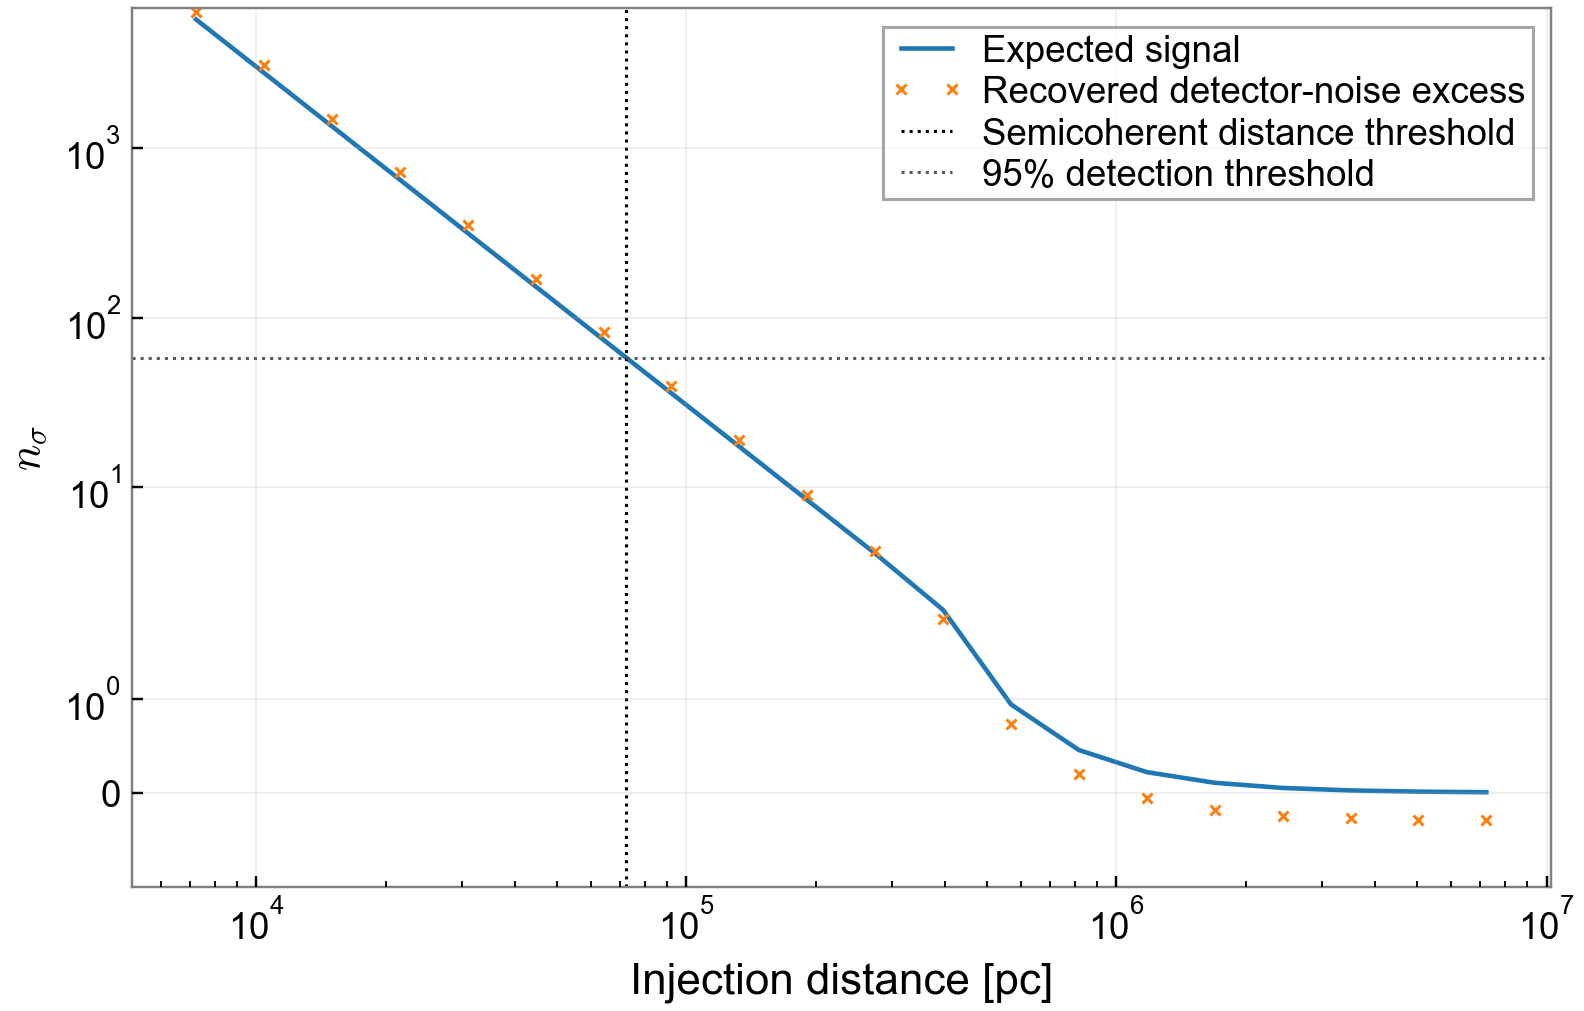
\includegraphics[width=0.8\columnwidth]{figs/z_vs_distance_detector_noise.png}
    \caption{
        DRAFT \nl{Need to remake this plot}
    }
    \label{fig:injection_vs_distance}
\end{figure}

%==========================================================================


%==========================================================================

\section{Computational cost}
\label{sec:cost}
The computational cost of the search is dominated by two stages: constructing the resampled spectra and evaluating the semicoherent stack-slide statistic. For each value of the coherent resampling parameter $\beta$, we compute NUFFTs over $N_{\rm seg} = \lceil T_{\rm obs}/T_{\rm coh}\rceil$ coherent segments, where $\lceil \cdot \rceil$ denotes the ceiling function. Each coherent segment contains $\lceil T_{\rm coh} \cdot f_{\rm samp}\rceil$ samples. If we fix the desired NUFFT accuracy, the computational cost scales as:
\begin{equation}
C_{\rm NUFFT}
\propto
N_\beta T_{\rm obs} f_{\rm samp}
\log\left(T_{\rm coh} f_{\rm samp}\right) .
\end{equation}
In practice, we can benchmark this directly. On a commercial Intel Core Ultra 7 255U CPU utilizing 4 threads, the current implementation is able to analyze $\mathcal{O}(10^6)$ 30s segments per hour so would compute all the NUFFT spectra in $\mathcal{O}(10^4)$ hours. This is parallelizable and we could expect speedups of one-two orders of magnitude for a GPU implementation. 

After the resampled spectra are generated, evaluating the StackSlide statistic is computationally simple and consists of reading powers from the resampled spectra and accumulating weighted sums. It is, therefore, expected to be limited by memory bandwidth. The average number of power reads per template, corresponding to the number of coherent segments spanned by a signal, is $\mathcal{O}(10^3)$. For a bank containing $\mathcal{O}(10^{10})$ templates, this requires $\mathcal{O}(10^{13})$ power reads, corresponding to approximately $20\,\mathrm{TB}$ of memory traffic when the powers are stored in half precision. As representative values, a CPU with dual-channel DDR5 memory can sustain approximately $50\,\mathrm{GB\,s^{-1}}$, while a modern consumer GPU with GDDR6X or GDDR7 memory can sustain approximately $500\,\mathrm{GB\,s^{-1}}$. These correspond to evaluation times of $\mathcal{O}(10^3)\,\mathrm{s}$ on a CPU and $\mathcal{O}(10^2)\,\mathrm{s}$ on a GPU.

A practical limitation is memory size, storing the resampled spectra requires:
\begin{equation}
M
=
N_\beta Tf_{\rm band}b ,
\end{equation}
where $b$ is the number of bytes stored per frequency bin. For half precision: $b=2$. With $T=1,{\rm yr}$, $N_\beta=69$, and $f_{\rm band}=20\,{\rm Hz}$, this gives
\begin{equation}
M \simeq 170\,{\rm GB}
\end{equation}
This exceeds the memory available on a single high-end GPU.

We therefore evaluate the stack-slide statistic in time blocks that fit in GPU memory. For a memory budget $M_{\rm GPU}$, the maximum block duration is approximately
\begin{equation}
T_{\rm block}
\simeq
\frac{M_{\rm GPU}}
{N_\beta (f_{\rm high}-f_{\rm low})b} .
\end{equation}
For $M_{\rm GPU}=80,{\rm GB}$, this corresponds to $T_{\rm block}\approx 165 \,{\rm days}$. Templates whose tracks lie entirely within a block require no additional memory movement. Templates crossing a block boundary can be handled by caching partial sums, which adds only a small memory overhead compared to storing the spectra themselves.

% \subsection{Vetos and follow up}

% \ls{I don't think this section is necessary. There is nothing new, and we are not doing a real search in this paper}

% Candidates are ranked by the semicoherent detection statistic and clustered in parameter space, with the loudest template retained from each cluster. The first veto is multi-detector coincidence: a viable candidate must have consistent parameters and compatible relative amplitudes across detectors, accounting for antenna responses and noise levels. Candidates significant in only one detector, or with inconsistent best-fit parameters, are rejected.

% We also apply time-frequency consistency tests. Since the signal is not monochromatic, intersections with known instrumental lines do not by themselves provide a sufficient veto. Instead, we test whether the accumulated power follows the expected frequency evolution and is distributed across the observing span. Candidates whose statistic is dominated by a small number of segments are rejected, as this behaviour is more consistent with transient artifacts than with a long-duration signal. Robustness is further tested by removing high-contribution segments, individual detectors, or flagged data-quality segments.

% Surviving candidates are followed up with increasingly sensitive configurations. The template grid is refined around the candidate, the coherent duration is increased, and the search is repeated with finer sampling of the relevant physical parameters. A genuine signal should remain localized in parameter space and increase in significance consistently with the improved coherent sensitivity. Final follow-ups include analyses with independent implementations or algorithms, alternative waveform models, and simulated injections. Where appropriate, the parameter space is expanded to include additional intrinsic or extrinsic parameters not varied in the initial search.


%==========================================================================

\section{Conclusion}
\label{sec:conclusion}
In this work, we have presented a novel implementation of resampling based on
type-I NUFFTs. The method evaluates the Fourier spectrum directly from samples
that are nonuniform in the transformed time coordinate, thereby combining the
resampling and Fourier-transform operations without constructing a uniformly
sampled intermediate time series. It therefore avoids the nearest-neighbour
interpolation and oversampling required by stroboscopic resampling. At
numerical accuracies representative of existing stroboscopic implementations,
our benchmarks show speedups of $\mathcal{O}(10)$--$\mathcal{O}(10^2)$. The precise gain
depends on the coherent-segment duration, computing hardware, and requested
numerical tolerance.

To demonstrate the applicability of this technique, we have constructed a
frequentist semicoherent search for long-duration inspirals from subsolar-mass
black-hole binaries, including systems that may be of primordial origin. The
estimated distance sensitivity extends beyond the Galactic Centre and, over
part of the parameter space, reaches Andromeda. Our computational estimates
indicate that the search is feasible with parallel computing resources and
that its performance could be improved further through GPU acceleration.
These results establish NUFFT-based resampling as an efficient foundation for
semicoherent searches for long-transient gravitational-wave
signals. 

%==========================================================================
\begin{acknowledgments}
We thank ...
This work is supported by the Australian Research Council Centre of Excellence for Gravitational Wave Discovery (OzGrav), Project Number CE230100016. 
L.S. is also supported by the Australian Research Council Discovery Early Career Researcher Award, Project Number DE240100206. 
\end{acknowledgments}  


\appendix
\section{Resampling and convolutions}
\label{sec:resampling_convolution}
Resampling requires evaluating the signal on a uniformly spaced time grid in the resampled time coordinate. This is achieved by interpolating from the non-uniform samples, with the interpolation rule specifying how neighbouring samples contribute to each point on the resampled grid. Equivalently, the interpolation may be represented as a convolution with an interpolation kernel.

The choice of interpolation kernel determines both the accuracy and computational cost of the resampling procedure. In the frequency domain, a kernel with a narrow spectral width is desirable in order to suppress contributions from aliased spectral replicas. A narrow kernel in the time-domain, however, is preferable because it reduces the number of neighbouring samples that must be evaluated for each interpolated point. These requirements are in tension, analogous to the familiar time-frequency tradeoff in the design of window functions. Prolate spheroidal wave functions provide near-optimal localization under such competing constraints. These wave functions, however, are computationally expensive to evaluate, making practical implementation with infeasible. Realistic choices of convolution kernel must also account for the computational cost of evaluating the kernel and deconvolution terms, and no universally optimal choice currently exists.

% \section{Computational performance}
% \label{sec:nufft_performance}
% \nl{Need to finish this}

% We now compare the computational cost of the stroboscopic resampling procedure with the NUFFT-based implementation introduced above. Let $N$ denote the length of the final resampled time series, or equivalently the number of Fourier modes required in the final spectrum. In stroboscopic resampling, the time series is first sampled at a higher rate such that it is an upsampled time series of length:
% \begin{equation}
% U = rN , ,
% \end{equation}
% where $r$ is the oversampling factor. Nearest-neighbour interpolation is then used to construct a uniformly sampled time series in the new time coordinate, after which a standard FFT is applied. The interpolation step requires scanning over the upsampled time series and has complexity $\mathcal{O}(U)$ so the total complexity is
% \begin{equation}
% C_\text{strobo} = \mathcal{O}(rN + N\log N) , .
% \end{equation}
% To first order the error of the FFT spectra scales linearly with the the interpolation error so is:
% \begin{equation}
% \epsilon_\text{strobo} = \mathcal{O}(1/r) , .
% \end{equation}
% Thus, improving the accuracy by one order of magnitude requires increasing the length of the upsampled time series by the same factor.

% For a NUFFT-based implementation, the non-uniformly sampled data in the resampled time coordinate are instead transformed directly into Fourier modes. In one dimensional timeseries the complexity given $N$ non-uniform points and output modes is:
% \begin{equation}
% C_\text{NUFFT} = \mathcal{O}\left(N|\log \epsilon| + N\log N\right) , ,
% \end{equation}
% where $\epsilon$ is the requested transform accuracy. Matching the accuracy of stroboscopic resampling:
% \begin{equation}
% C_\text{NUFFT} = \mathcal{O}\left(N\log r + N\log N\right) , .
% \end{equation}
% Stroboscopic methods therefore linearly in the oversampling factor $r$, whereas the NUFFT pays only logarithmically in the target accuracy.

% The expected asymptotic speedup at fixed accuracy is:
% \begin{equation}
% \frac{C_\text{strobo}}{C_\text{NUFFT}}
% \sim
% \frac{r + \log N}{\log r + \log N} , .
% \label{eq:nufft_speedup_scaling}
% \end{equation}
% In the high-accuracy regime relevant for stroboscopic resampling, the upsampled time series is typically much longer than the final FFT length contribution, i.e:
% \begin{equation}
% U \gg N\log N
% \quad \Longleftrightarrow \quad
% r \gg \log N , .
% \end{equation}
% For example, for $N \sim 10^6$--$10^8$ if nearest-neighbour interpolation requires $r \sim 10^2$ to reach the desired accuracy, then the cost of scanning the upsampled time series dominates the stroboscopic method. In this regime Eq. \eqref{eq:nufft_speedup_scaling} gives an expected speedup of order 5--50.

% NUFFT algorithms generally all have complexity,
% \begin{equation}
% \mathcal{O}\left(N|\log\epsilon| + N\log N\right) , ,
% \end{equation}
% in one dimension, but their practical performance depends on the kernel used for spreading/interpolation, the width of the kernel support, memory access patterns, precomputation, threading, vectorization, and cache behaviour. These factors can change the prefactor by more than an order of magnitude even when the formal scaling is unchanged.

% The fiNUFFT implementation used in this work uses the ``exponential of a semicircle'' kernel,
% \begin{equation}
% \varphi(x) = \exp\left[\beta \sqrt{1-x^2}\right] , ,
% \qquad |x| \leq 1 , ,
% \end{equation}
% with compact support and an efficient load-balanced spreading implementation \cite{2019SJSC...41C.479B}. This kernel has near-optimal exponential convergence in the kernel width, comparable to Kaiser--Bessel and prolate spheroidal wavefunction kernels. As a rough comparison, if an order-8 Dirichlet-style interpolation stencil requires eight neighbouring grid points per sample, while FINUFFT achieves the same target precision with an effective kernel width of $w\simeq 6$--$7$, the raw spreading work alone would be smaller by a factor of approximately
% \begin{equation}
% \frac{8}{w} \simeq 1.1\text{--}1.3 , .
% \end{equation}
% This estimate captures only the direct stencil-width contribution. In practice, the speedup can be larger or smaller depending on the cost of evaluating the kernel, whether interpolation weights are precomputed, how well the implementation vectorizes, and how efficiently memory is accessed. The main computational gain in our application therefore comes not from a small change in kernel order alone, but from replacing the explicit construction and traversal of an upsampled time series of length $U=rN$ with a NUFFT whose accuracy cost grows only as $\log r$.

%%%%%%%%%%%%%%%%%%%%%%%%%%%%%%%%%%%%%%%%%%%%%%%%%%%%%%%%%%%%%%%%%%%%%%%%%%%%%%%
\def\bibsection{\section*{References}}
%%%%%%%%%%%%%%%%%%%%%%%%%%%%%%%%%%%%%%%%%%%%%%%%%%%%%%%%%%%%%%%%%%%%%%%%%%%%%%%
\bibliographystyle{apsrev4-2-author-truncate.bst}
\bibliography{zotero.bib}


\end{document}
